\documentclass[aspectratio=169]{beamer}\usepackage[]{graphicx}\usepackage[]{color}
% maxwidth is the original width if it is less than linewidth
% otherwise use linewidth (to make sure the graphics do not exceed the margin)
\makeatletter
\def\maxwidth{ %
  \ifdim\Gin@nat@width>\linewidth
    \linewidth
  \else
    \Gin@nat@width
  \fi
}
\makeatother

\definecolor{fgcolor}{rgb}{0.345, 0.345, 0.345}
\newcommand{\hlnum}[1]{\textcolor[rgb]{0.686,0.059,0.569}{#1}}%
\newcommand{\hlstr}[1]{\textcolor[rgb]{0.192,0.494,0.8}{#1}}%
\newcommand{\hlcom}[1]{\textcolor[rgb]{0.678,0.584,0.686}{\textit{#1}}}%
\newcommand{\hlopt}[1]{\textcolor[rgb]{0,0,0}{#1}}%
\newcommand{\hlstd}[1]{\textcolor[rgb]{0.345,0.345,0.345}{#1}}%
\newcommand{\hlkwa}[1]{\textcolor[rgb]{0.161,0.373,0.58}{\textbf{#1}}}%
\newcommand{\hlkwb}[1]{\textcolor[rgb]{0.69,0.353,0.396}{#1}}%
\newcommand{\hlkwc}[1]{\textcolor[rgb]{0.333,0.667,0.333}{#1}}%
\newcommand{\hlkwd}[1]{\textcolor[rgb]{0.737,0.353,0.396}{\textbf{#1}}}%
\let\hlipl\hlkwb

\usepackage{framed}
\makeatletter
\newenvironment{kframe}{%
 \def\at@end@of@kframe{}%
 \ifinner\ifhmode%
  \def\at@end@of@kframe{\end{minipage}}%
  \begin{minipage}{\columnwidth}%
 \fi\fi%
 \def\FrameCommand##1{\hskip\@totalleftmargin \hskip-\fboxsep
 \colorbox{shadecolor}{##1}\hskip-\fboxsep
     % There is no \\@totalrightmargin, so:
     \hskip-\linewidth \hskip-\@totalleftmargin \hskip\columnwidth}%
 \MakeFramed {\advance\hsize-\width
   \@totalleftmargin\z@ \linewidth\hsize
   \@setminipage}}%
 {\par\unskip\endMakeFramed%
 \at@end@of@kframe}
\makeatother

\definecolor{shadecolor}{rgb}{.97, .97, .97}
\definecolor{messagecolor}{rgb}{0, 0, 0}
\definecolor{warningcolor}{rgb}{1, 0, 1}
\definecolor{errorcolor}{rgb}{1, 0, 0}
\newenvironment{knitrout}{}{} % an empty environment to be redefined in TeX

\usepackage{alltt}
\usepackage{multirow}
%\usecolortheme{beaver}
%\usecolortheme[RGB={129,3,3}]{structure}
\usetheme{CambridgeUS}
\usecolortheme{seahorse}

% Standard header (will need to change date!)
\title[GEOG 5680 Summer '20]{GEOG 5680\\Introduction to R}
\subtitle[Intro]{09: Probabilities and Inference tests}
\author[S. Brewer]{Simon Brewer}
\institute[Univ. Utah]{
  Geography Department\\
  University of Utah\\
  Salt Lake City, Utah 84112\\[1ex]
  \texttt{simon.brewer@geog.utah.edu}
}
\date[May 04, 2020]{May 04, 2020}
\IfFileExists{upquote.sty}{\usepackage{upquote}}{}
\begin{document}


%--- the titlepage frame -------------------------%
\begin{frame}
  \titlepage
\end{frame}

% %--- Slide ----------------%
% \begin{frame}{Outline}
% \begin{itemize}
%   \item Probability (in R)
%   \item Statistical distributions
%   \item Statistical inference
%   \item $t$-test example
%   \item ANOVA and other standard tests
% \end{itemize}
% \end{frame}
% 
\section{Probability}
%-----frame-----%
\begin{frame}{Probability}
What is this thing called probability?
\begin{itemize}
  \item Mathematical description of uncertainty
  \item Tightly linked to statistics for inference
  \begin{itemize}
    \item Model of population from samples
  \end{itemize}
  \item Several functions in R for estimating probability
  \item Also found as part of the inference in test in other functions (e.g. ANOVA, linear models, etc)
\end{itemize}
\end{frame}

%-----frame-----%
\begin{frame}{Probability}
What is this thing called probability?
\begin{itemize}
  \item Probability shows what \emph{outcomes} might occur given a \emph{model}
  \begin{itemize}
    \item Given the animal, what are the footprints?
  \end{itemize}
  \item<2-> Statistics show what \emph{models} might result in a given \emph{outcome}
  \begin{itemize}
    \item Given the footprints, what is the animal?
  \end{itemize}
\end{itemize}
\end{frame}

% %-----frame-----%
% \begin{frame}{Probability}
% Some vocabulary
% \begin{itemize}
%   \item Outcome
%   \begin{itemize}
%     \item Result of an experiment
%   \end{itemize}
%   \item Sample space
%   \begin{itemize}
%     \item All possible outcomes of an experiment
%   \end{itemize}
%   \item Random variable
%   \begin{itemize}
%     \item Translation of sample space into simpler numerical value
%     \item E.g. How many heads in 10 coin tosses
%     \item Sample space ($\Omega$) has $2^{10}$ entries
%     \item Random variable ($X$) has just 11: $\{ 0,1,2,3,4,5,6,7,8,9,10 \}$
%   \end{itemize}
% \end{itemize}
% \end{frame}
% 
% %-----frame-----%
% \begin{frame}{Probability}
% Some vocabulary
% \begin{itemize}
%   \item Probability
%   \begin{itemize}
%     \item Chance of a given outcome ($x_i$) in random variable occuring
%     \item $0 \le p(x_i) \le 1$
%   \end{itemize}
%   \item Probability distribution 
%   \begin{itemize}
%     \item List of probabilities for all possible outcomes defined in random variable
%     \item $\sum p(x_i) = 1$
%   \end{itemize}
% \end{itemize}
% \end{frame}
% 
% %-----frame-----%
% \begin{frame}{Probability mass function}
% \begin{columns}
%   \begin{column}{0.5\textwidth}
%   \begin{itemize}
%     \item Probability mass function
%     \item Used with discrete variables (binary, counts, etc)
%     \item Value given is probability for that outcome
%     \item E.g. $p(2)=$ dpois(2,4)
%   \end{itemize}
%   \end{column}
%   \begin{column}{0.5\textwidth}
% <<echo=FALSE>>=
% set.seed(8888)
% #x1 = rpois(100, 4)
% x1 = seq(0,12)
% d1 = dpois(x1, 4)
% barplot(d1, names.arg = x1, main="Number of trees (prob. mass)")
% abline(h=dpois(2,4), lty=2)
% @
%   \end{column}
% \end{columns}
% \end{frame}
% 
% %-----frame-----%
% \begin{frame}{Probability density function}
% \begin{columns}
%   \begin{column}{0.5\textwidth}
%   \begin{itemize}
%     \item Probability density function
%     \item Used with continuous variables
%     \item Value given is \emph{density} of probability, not probability
%   \end{itemize}
%   \end{column}
%   \begin{column}{0.5\textwidth}
% <<echo=FALSE>>=
% x2 = rnorm(100, 160,15)
% qq = seq(0,250,1)
% dd = dnorm(qq,160,15)
% plot(qq, dd, main="Student height (prob. density)", type='l', lwd=2, 
%      xlab="cm", ylab="D", xlim=c(100,220))
% @
%   \end{column}
% \end{columns}
% \end{frame}
% 
% %-----frame-----%
% \begin{frame}{Probability density function}
% \begin{columns}
%   \begin{column}{0.5\textwidth}
%   \begin{itemize}
%     \item Value given is \emph{density} of probability, not probability
%     \item Use integrals to estimate the probability of being less than (or greater than) a given value
%     \item E.g. $p(<155)=$ round(pnorm(155, 160, 15, lower.tail=TRUE),4)
%   \end{itemize}
%   \end{column}
%   \begin{column}{0.5\textwidth}
% <<echo=FALSE>>=
% plot(qq, dd, main="Student height (prob. density)", type='l', lwd=2, 
%      xlab="cm", ylab="D", xlim=c(100,220))
% xvals <- seq(50,155,length=100)
% dvals <- dnorm(xvals,160,15)
% polygon(c(xvals,rev(xvals)),c(rep(0,100),rev(dvals)),col="lightgray")
% text(120,0.02,
%      paste("p(<155)=",round(pnorm(155, 160, 15, lower.tail=TRUE),4)))
% @
%   \end{column}
% \end{columns}
% \end{frame}
% 
% %-----frame-----%
% \begin{frame}{Probability density function}
% \begin{columns}
%   \begin{column}{0.5\textwidth}
%   \begin{itemize}
%     \item Value given is \emph{density} of probability, not probability
%     \item Use integrals to estimate the probability of being less than (or greater than) a given value
%     \item E.g. $p(>180)=$ round(pnorm(180, 160, 15, lower.tail=FALSE),4)
%   \end{itemize}
%   \end{column}
%   \begin{column}{0.5\textwidth}
% <<echo=FALSE>>=
% plot(qq, dd, main="Student height (prob. density)", type='l', lwd=2, 
%      xlab="cm", ylab="D", xlim=c(100,220))
% xvals <- seq(180,250,length=100)
% dvals <- dnorm(xvals,160,15)
% polygon(c(xvals,rev(xvals)),c(rep(0,100),rev(dvals)),col="lightgray")
% text(120,0.02,
%      paste("p(>180)=",round(pnorm(180, 160, 15, lower.tail=FALSE),4)))
% @
%   \end{column}
% \end{columns}
% \end{frame}
% 
\section{Distributions in R}
%--- Slide ----------------%
\begin{frame}{Distributions in R}
\begin{itemize}
  \item R comes as standard with approx. 20 well-known probability distribution functions
  \item Including normal, uniform, binomial, log-normal, beta, gamma, $t$, $F$, $\chi^2$ etc
  \item Add-on packages include approx 100+ extra distributions
  \item Most distribution come with four functions:
  \begin{itemize}
    \item \texttt{d*} --- density functions (e.g. \texttt{dnorm()})
    \item \texttt{p*} --- probability distribution functions (e.g. \texttt{pnorm()})
    \item \texttt{q*} --- quantile functions (e.g. \texttt{qnorm()})
    \item \texttt{r*} --- random number generation (e.g. \texttt{rnorm()})
  \end{itemize}
  \item Look at examples with Poisson (discrete, count) and normal (continuous)
\end{itemize}
\end{frame}

\subsection{Poisson distribution}
%-----frame-----%
\begin{frame}[fragile]{Poisson distribution}
\begin{columns}
  \begin{column}{0.5\textwidth}
  \begin{itemize}
    \item Count data ($\lambda$ = mean count)
    \item \texttt{d*}: density function, gives the height of the density curve for a given value
    \item E.g what is the probability of getting 6 trees in a quadrat?
  \end{itemize}
\begin{knitrout}\scriptsize
\definecolor{shadecolor}{rgb}{0.969, 0.969, 0.969}\color{fgcolor}\begin{kframe}
\begin{alltt}
\hlkwd{dpois}\hlstd{(}\hlnum{6}\hlstd{,}\hlkwc{lambda}\hlstd{=}\hlnum{4}\hlstd{)}
\end{alltt}
\begin{verbatim}
## [1] 0.1041956
\end{verbatim}
\end{kframe}
\end{knitrout}
  \end{column}
  \begin{column}{0.5\textwidth}
\begin{knitrout}\scriptsize
\definecolor{shadecolor}{rgb}{0.969, 0.969, 0.969}\color{fgcolor}
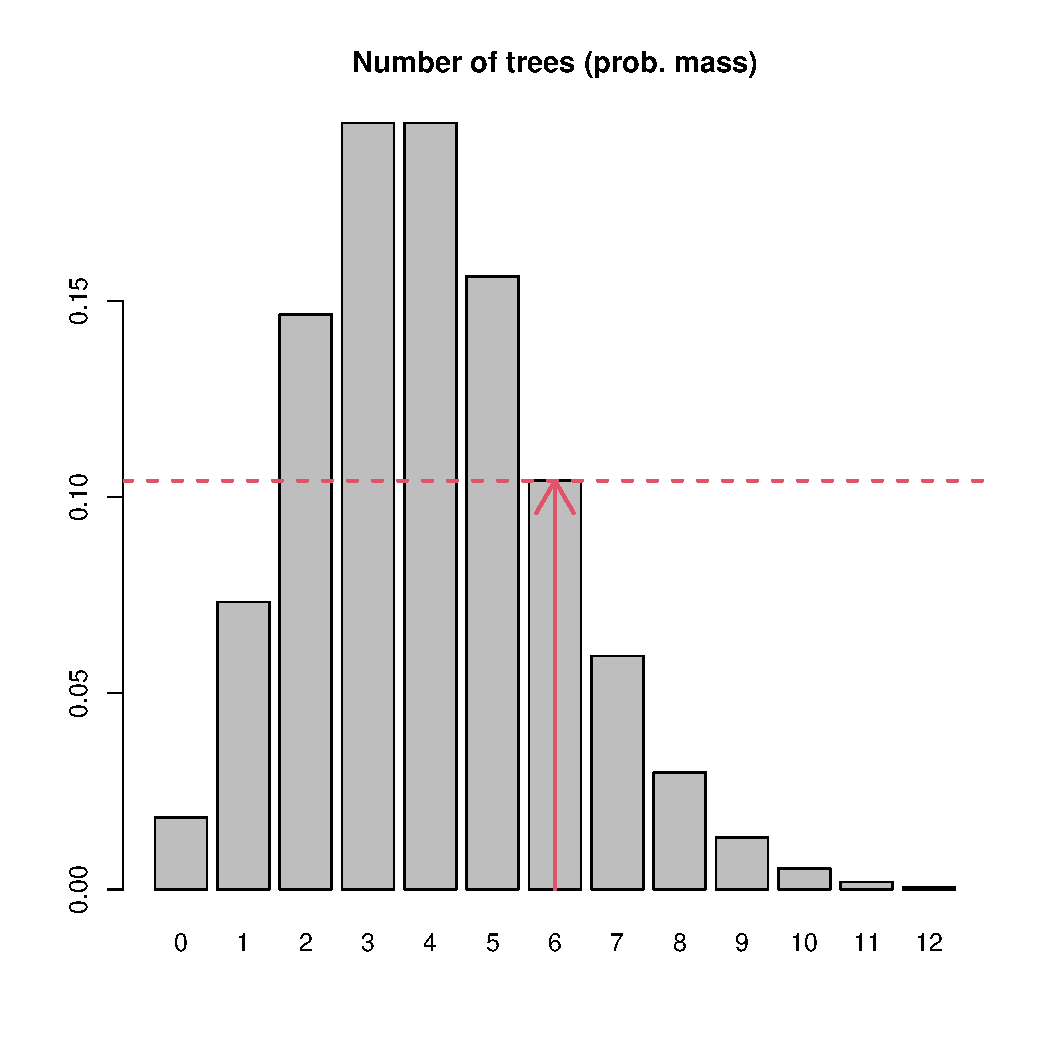
\includegraphics[width=\maxwidth]{figure/unnamed-chunk-2-1} 

\end{knitrout}
  \end{column}
\end{columns}
\end{frame}

%-----frame-----%
\begin{frame}[fragile]{Poisson distribution}
\begin{columns}
  \begin{column}{0.5\textwidth}
  \begin{itemize}
    \item Count data ($\lambda$ = mean count)
    \item \texttt{p*}: probability dist. function, gives the integral above or below that value
    \item E.g what is the probability of getting $\le 6$ trees in a quadrat?
  \end{itemize}
\begin{knitrout}\scriptsize
\definecolor{shadecolor}{rgb}{0.969, 0.969, 0.969}\color{fgcolor}\begin{kframe}
\begin{alltt}
\hlkwd{ppois}\hlstd{(}\hlnum{6}\hlstd{,}\hlkwc{lambda}\hlstd{=}\hlnum{4}\hlstd{,}
      \hlkwc{lower.tail} \hlstd{=} \hlnum{TRUE}\hlstd{)}
\end{alltt}
\begin{verbatim}
## [1] 0.889326
\end{verbatim}
\end{kframe}
\end{knitrout}
  \end{column}
  \begin{column}{0.5\textwidth}
\begin{knitrout}\scriptsize
\definecolor{shadecolor}{rgb}{0.969, 0.969, 0.969}\color{fgcolor}
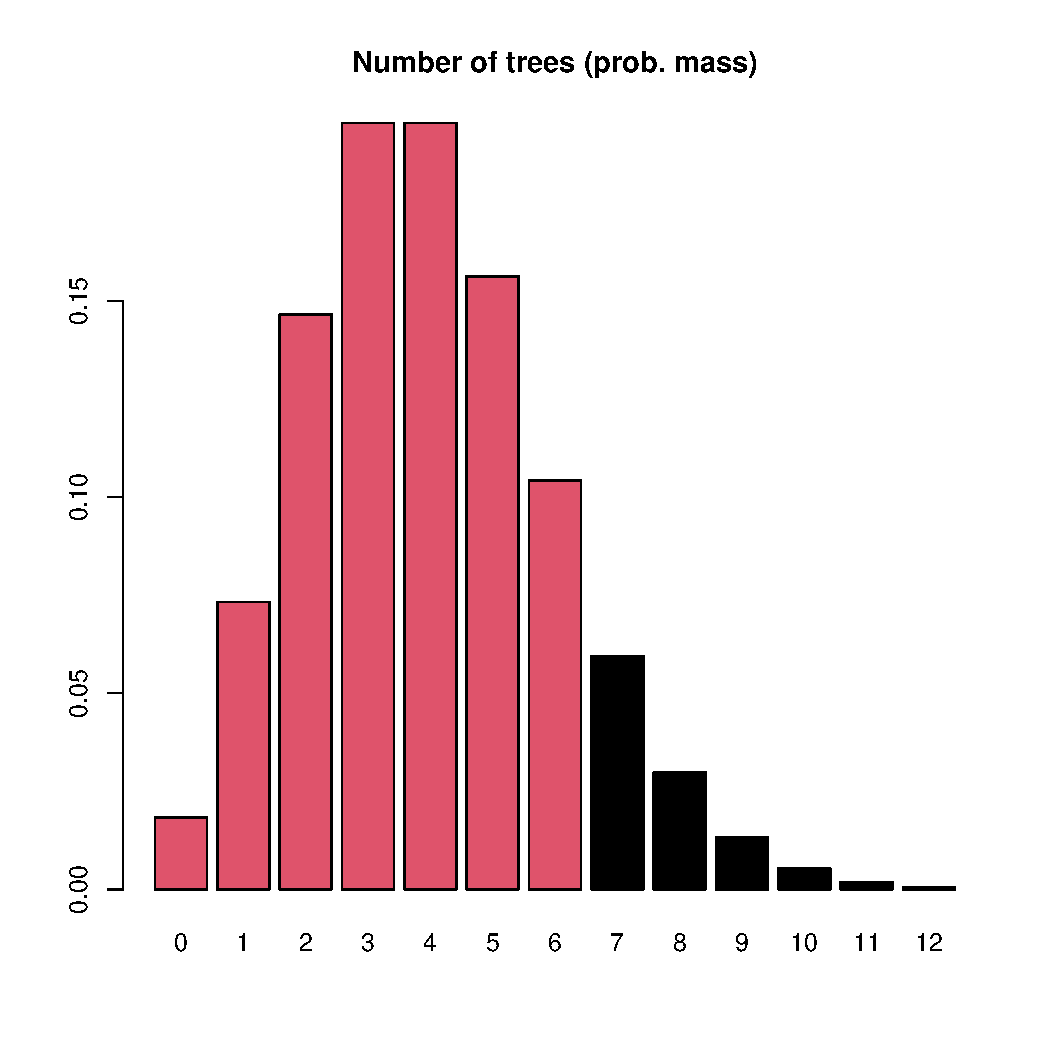
\includegraphics[width=\maxwidth]{figure/unnamed-chunk-4-1} 

\end{knitrout}
  \end{column}
\end{columns}
\end{frame}

%-----frame-----%
\begin{frame}[fragile]{Poisson distribution}
\begin{columns}
  \begin{column}{0.5\textwidth}
  \begin{itemize}
    \item Count data ($\lambda$ = mean count)
    \item \texttt{q*}: quantile function, gives the values of $X$ corresponding to a percentile probability
    \item E.g how many trees do we expect at the 10 percentile of the distribution?
  \end{itemize}
\begin{knitrout}\scriptsize
\definecolor{shadecolor}{rgb}{0.969, 0.969, 0.969}\color{fgcolor}\begin{kframe}
\begin{alltt}
\hlkwd{qpois}\hlstd{(}\hlnum{0.1}\hlstd{,}\hlkwc{lambda}\hlstd{=}\hlnum{4}\hlstd{)}
\end{alltt}
\begin{verbatim}
## [1] 2
\end{verbatim}
\end{kframe}
\end{knitrout}
  \end{column}
  \begin{column}{0.5\textwidth}
\begin{knitrout}\scriptsize
\definecolor{shadecolor}{rgb}{0.969, 0.969, 0.969}\color{fgcolor}
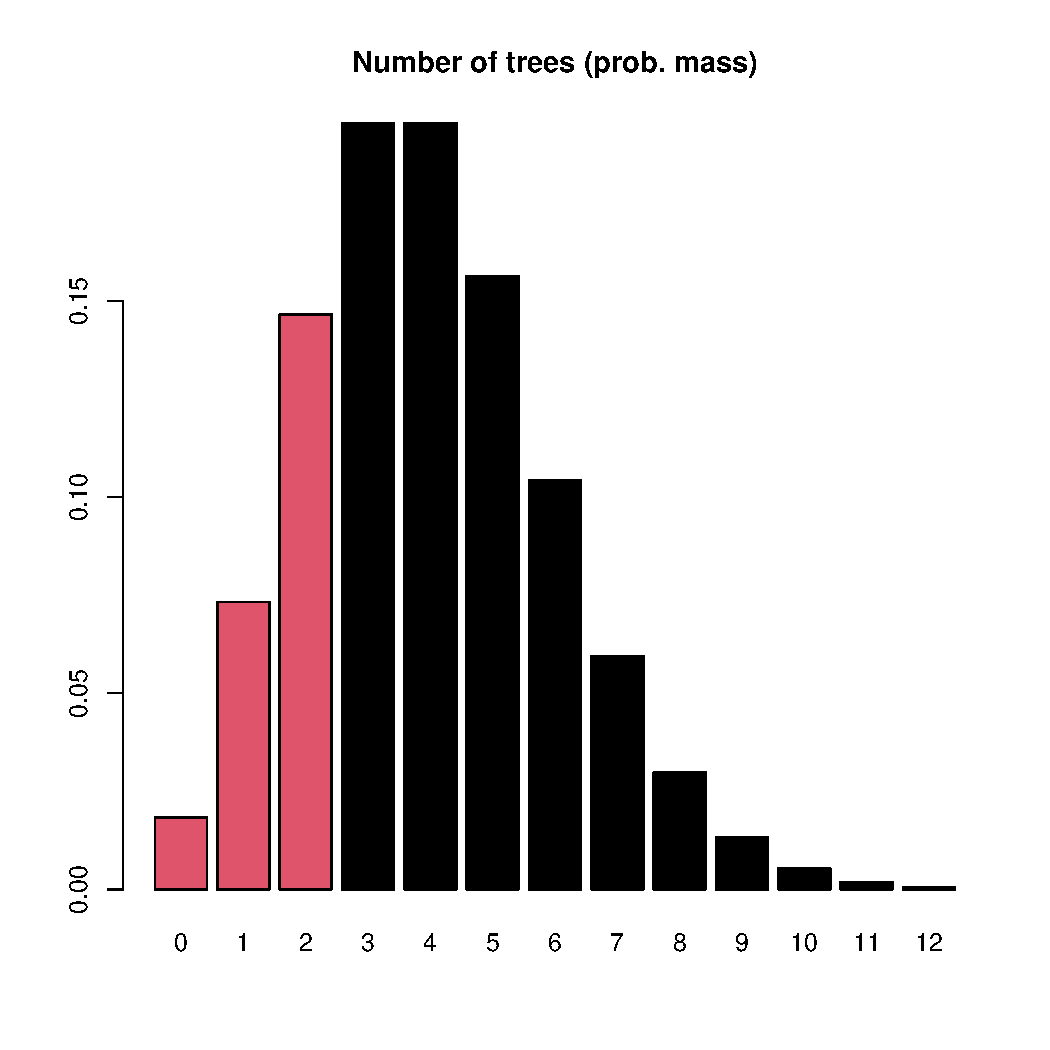
\includegraphics[width=\maxwidth]{figure/unnamed-chunk-6-1} 

\end{knitrout}
  \end{column}
\end{columns}
\end{frame}

%-----frame-----%
\begin{frame}[fragile]{Poisson distribution}
\begin{columns}
  \begin{column}{0.5\textwidth}
  \begin{itemize}
    \item Count data ($\lambda$ = mean count)
    \item \texttt{q*}: quantile function, gives the values of $X$ corresponding to a percentile probability
    \item E.g what is the 95\% CI on the number of trees we expect?
  \end{itemize}
\begin{knitrout}\scriptsize
\definecolor{shadecolor}{rgb}{0.969, 0.969, 0.969}\color{fgcolor}\begin{kframe}
\begin{alltt}
\hlkwd{qpois}\hlstd{(}\hlkwd{c}\hlstd{(}\hlnum{0.025}\hlstd{,}\hlnum{0.975}\hlstd{),}\hlkwc{lambda}\hlstd{=}\hlnum{4}\hlstd{)}
\end{alltt}
\begin{verbatim}
## [1] 1 8
\end{verbatim}
\end{kframe}
\end{knitrout}
  \end{column}
  \begin{column}{0.5\textwidth}
\begin{knitrout}\scriptsize
\definecolor{shadecolor}{rgb}{0.969, 0.969, 0.969}\color{fgcolor}
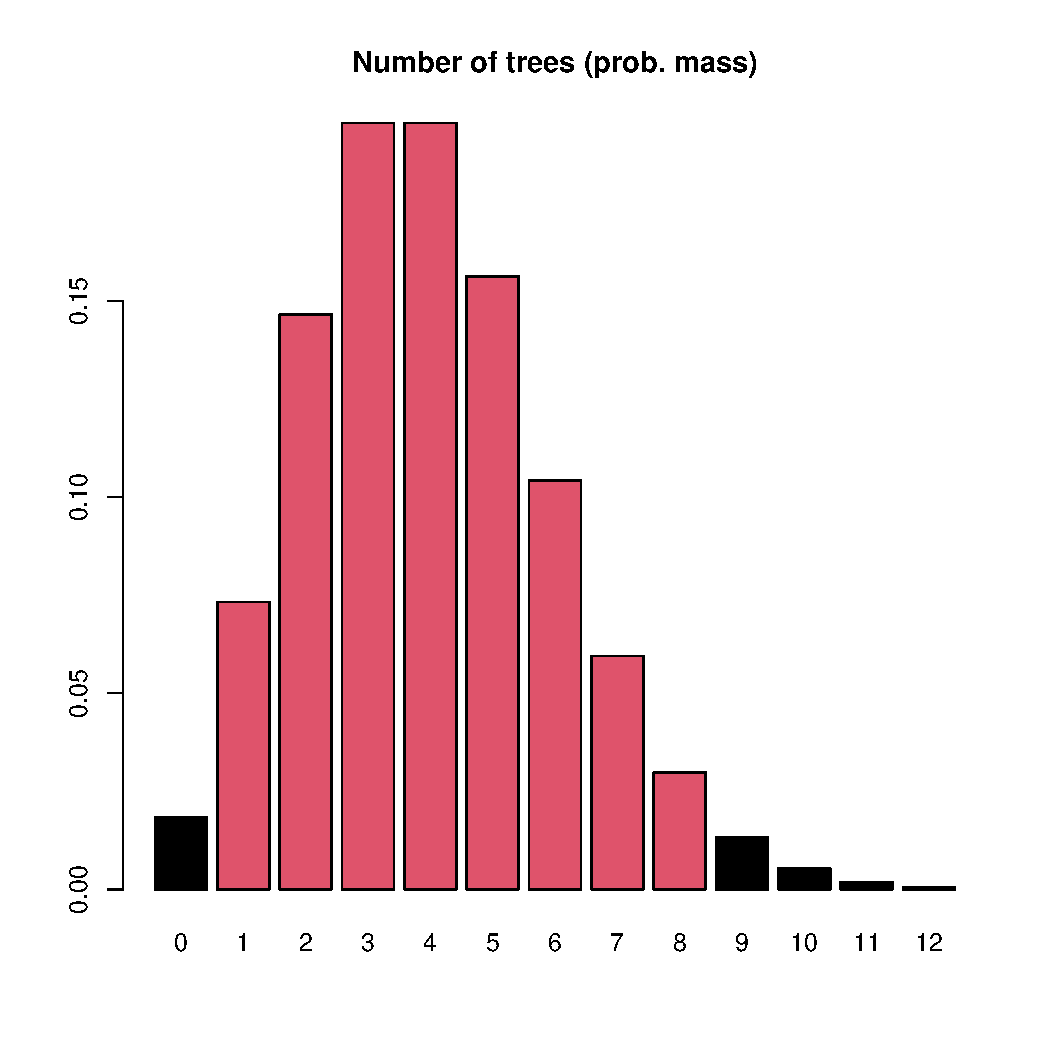
\includegraphics[width=\maxwidth]{figure/unnamed-chunk-8-1} 

\end{knitrout}
  \end{column}
\end{columns}
\end{frame}

%-----frame-----%
\begin{frame}[fragile]{Poisson distribution}
\begin{columns}
  \begin{column}{0.5\textwidth}
  \begin{itemize}
    \item Count data ($\lambda$ = mean count)
    \item \texttt{r*}: random function, generates random samples from the distribution
    \item E.g how many trees might be found in the next four plots?
  \end{itemize}
\begin{knitrout}\scriptsize
\definecolor{shadecolor}{rgb}{0.969, 0.969, 0.969}\color{fgcolor}\begin{kframe}
\begin{alltt}
\hlkwd{rpois}\hlstd{(}\hlnum{4}\hlstd{,}\hlkwc{lambda}\hlstd{=}\hlnum{4}\hlstd{)}
\end{alltt}
\begin{verbatim}
## [1] 4 4 6 3
\end{verbatim}
\begin{alltt}
\hlkwd{rpois}\hlstd{(}\hlnum{4}\hlstd{,}\hlkwc{lambda}\hlstd{=}\hlnum{4}\hlstd{)}
\end{alltt}
\begin{verbatim}
## [1] 4 5 4 2
\end{verbatim}
\end{kframe}
\end{knitrout}
  \end{column}
  \begin{column}{0.5\textwidth}
\begin{knitrout}\scriptsize
\definecolor{shadecolor}{rgb}{0.969, 0.969, 0.969}\color{fgcolor}
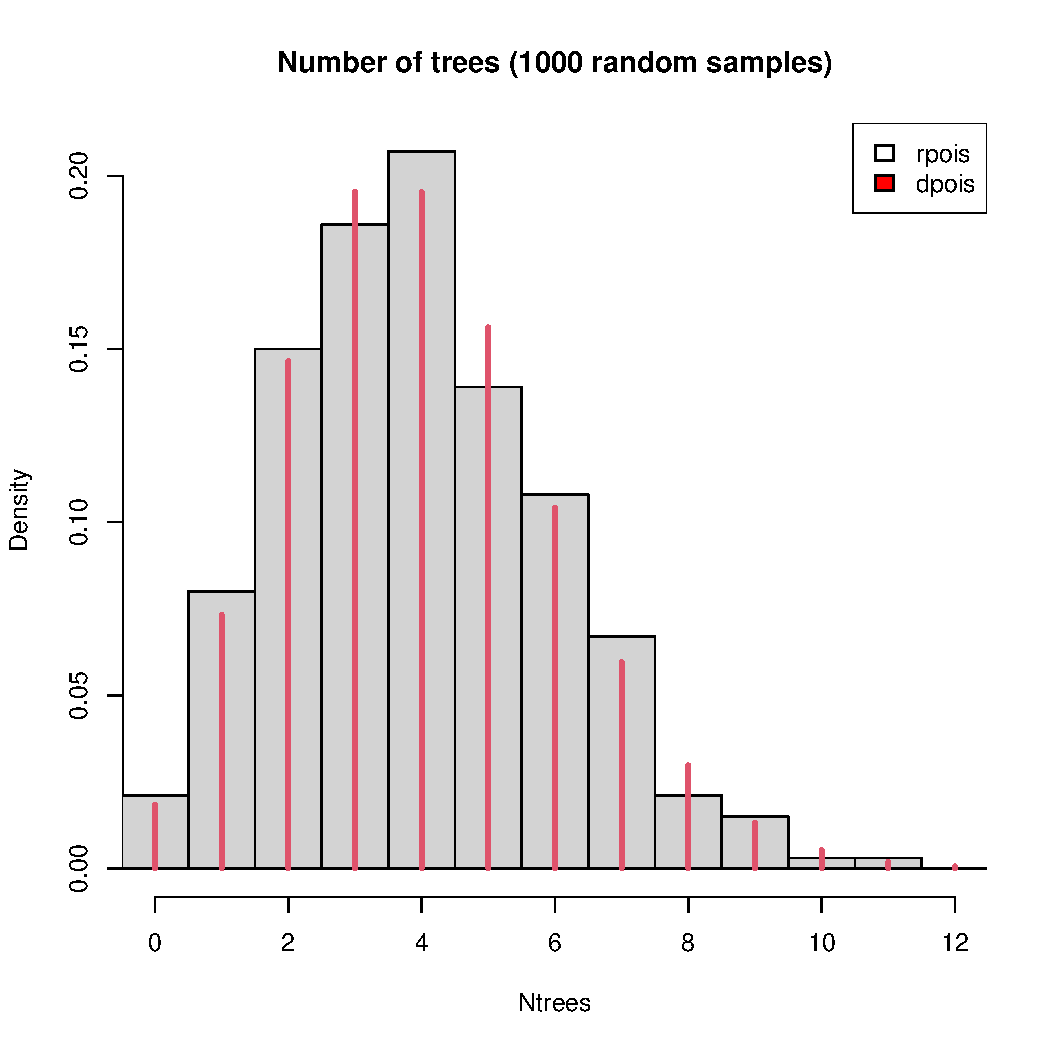
\includegraphics[width=\maxwidth]{figure/unnamed-chunk-10-1} 

\end{knitrout}
  \end{column}
\end{columns}
\end{frame}

\subsection{Normal distribution}
%-----frame-----%
\begin{frame}[fragile]{Normal distribution}
\begin{columns}
  \begin{column}{0.5\textwidth}
  \begin{itemize}
    \item Continuous data ($\mu$ = mean, $\sigma$ = std.dev.)
    \item \texttt{d*}: density function, gives the height of the density curve for a given value
    \item E.g what is the probability density for a height of 150cm?
  \end{itemize}
\begin{knitrout}\scriptsize
\definecolor{shadecolor}{rgb}{0.969, 0.969, 0.969}\color{fgcolor}\begin{kframe}
\begin{alltt}
\hlkwd{dnorm}\hlstd{(}\hlnum{150}\hlstd{,}\hlkwc{mean} \hlstd{=} \hlnum{160}\hlstd{,} \hlkwc{sd}\hlstd{=}\hlnum{15}\hlstd{)}
\end{alltt}
\begin{verbatim}
## [1] 0.02129653
\end{verbatim}
\end{kframe}
\end{knitrout}
  \end{column}
  \begin{column}{0.5\textwidth}
\begin{knitrout}\scriptsize
\definecolor{shadecolor}{rgb}{0.969, 0.969, 0.969}\color{fgcolor}
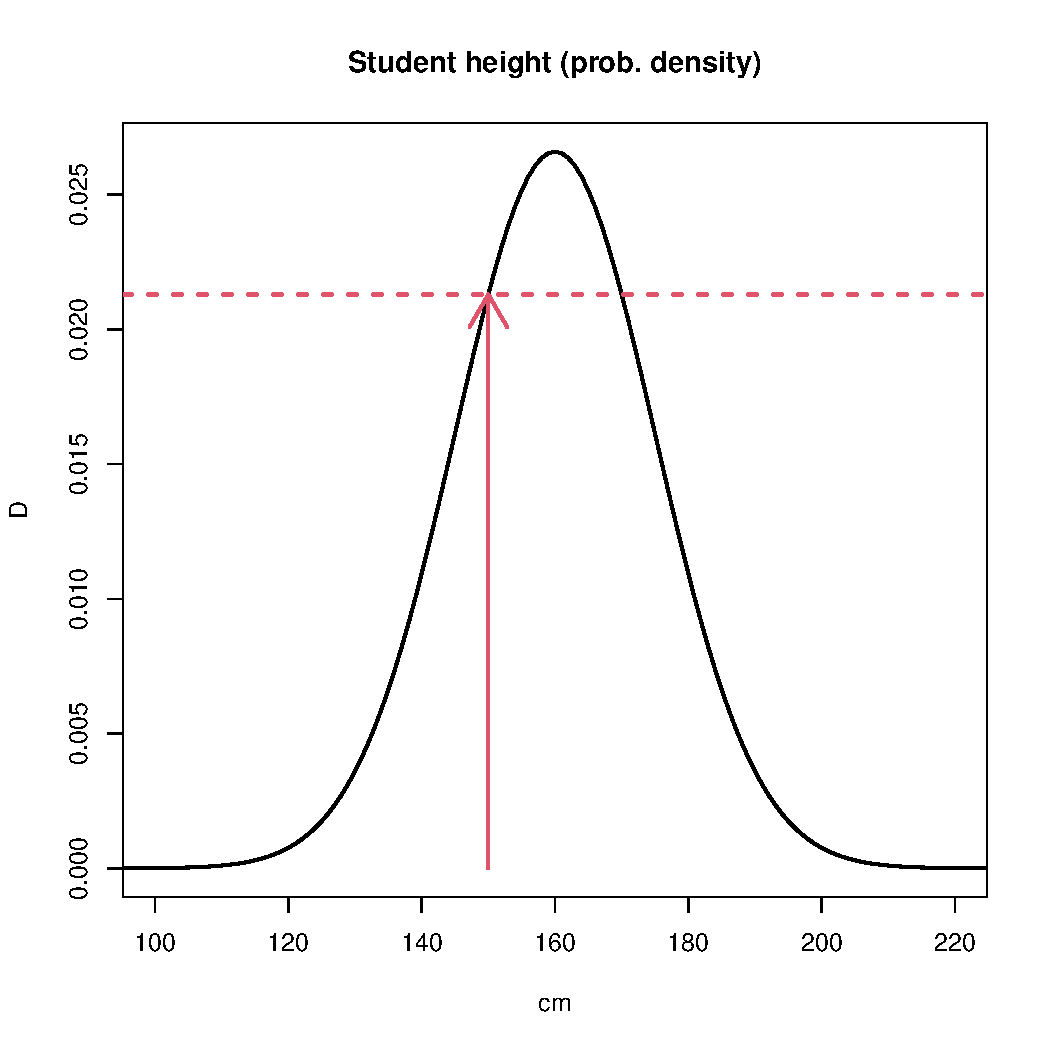
\includegraphics[width=\maxwidth]{figure/unnamed-chunk-12-1} 

\end{knitrout}
  \end{column}
\end{columns}
\end{frame}

%-----frame-----%
\begin{frame}[fragile]{Normal distribution}
\begin{columns}
  \begin{column}{0.5\textwidth}
  \begin{itemize}
    \item Continuous data ($\mu$ = mean, $\sigma$ = std.dev.)
    \item \texttt{p*}: probability dist. function, gives the integral above or below that value
    \item E.g what is the probability of a student being smaller than 140cm?
  \end{itemize}
\begin{knitrout}\scriptsize
\definecolor{shadecolor}{rgb}{0.969, 0.969, 0.969}\color{fgcolor}\begin{kframe}
\begin{alltt}
\hlkwd{pnorm}\hlstd{(}\hlnum{140}\hlstd{,} \hlnum{160}\hlstd{,} \hlnum{15}\hlstd{,}
      \hlkwc{lower.tail} \hlstd{=} \hlnum{TRUE}\hlstd{)}
\end{alltt}
\begin{verbatim}
## [1] 0.09121122
\end{verbatim}
\end{kframe}
\end{knitrout}
  \end{column}
  \begin{column}{0.5\textwidth}
\begin{knitrout}\scriptsize
\definecolor{shadecolor}{rgb}{0.969, 0.969, 0.969}\color{fgcolor}
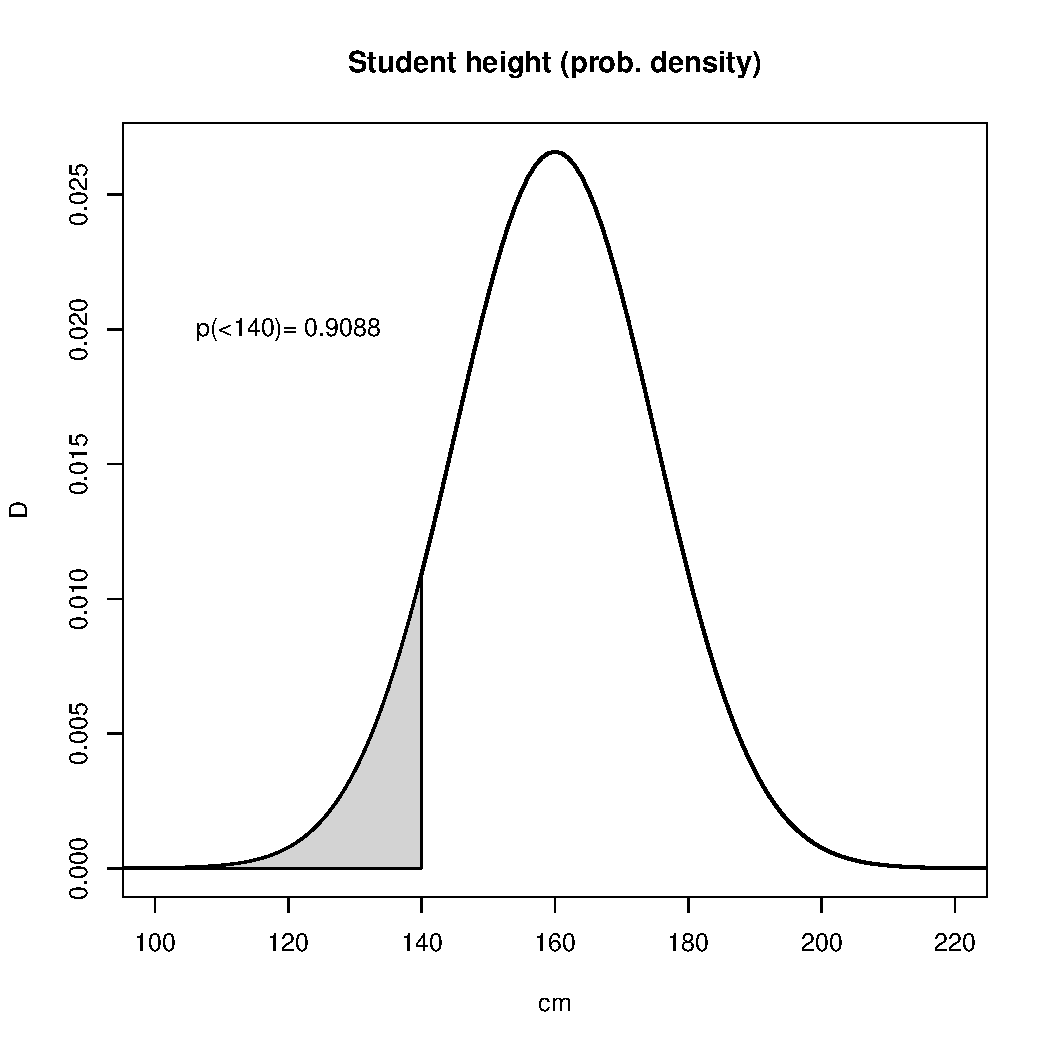
\includegraphics[width=\maxwidth]{figure/unnamed-chunk-14-1} 

\end{knitrout}
  \end{column}
\end{columns}
\end{frame}

%-----frame-----%
\begin{frame}[fragile]{Normal distribution}
\begin{columns}
  \begin{column}{0.5\textwidth}
  \begin{itemize}
    \item Continuous data ($\mu$ = mean, $\sigma$ = std.dev.)
    \item \texttt{q*}: quantile function, gives the values of $X$ corresponding to a percentile probability
    \item E.g what cutoff in height gives me the top $5\%$ of students?
  \end{itemize}
\begin{knitrout}\scriptsize
\definecolor{shadecolor}{rgb}{0.969, 0.969, 0.969}\color{fgcolor}\begin{kframe}
\begin{alltt}
\hlkwd{qnorm}\hlstd{(}\hlnum{0.95}\hlstd{,} \hlnum{160}\hlstd{,} \hlnum{15}\hlstd{)}
\end{alltt}
\begin{verbatim}
## [1] 184.6728
\end{verbatim}
\end{kframe}
\end{knitrout}
  \end{column}
  \begin{column}{0.5\textwidth}
\begin{knitrout}\scriptsize
\definecolor{shadecolor}{rgb}{0.969, 0.969, 0.969}\color{fgcolor}
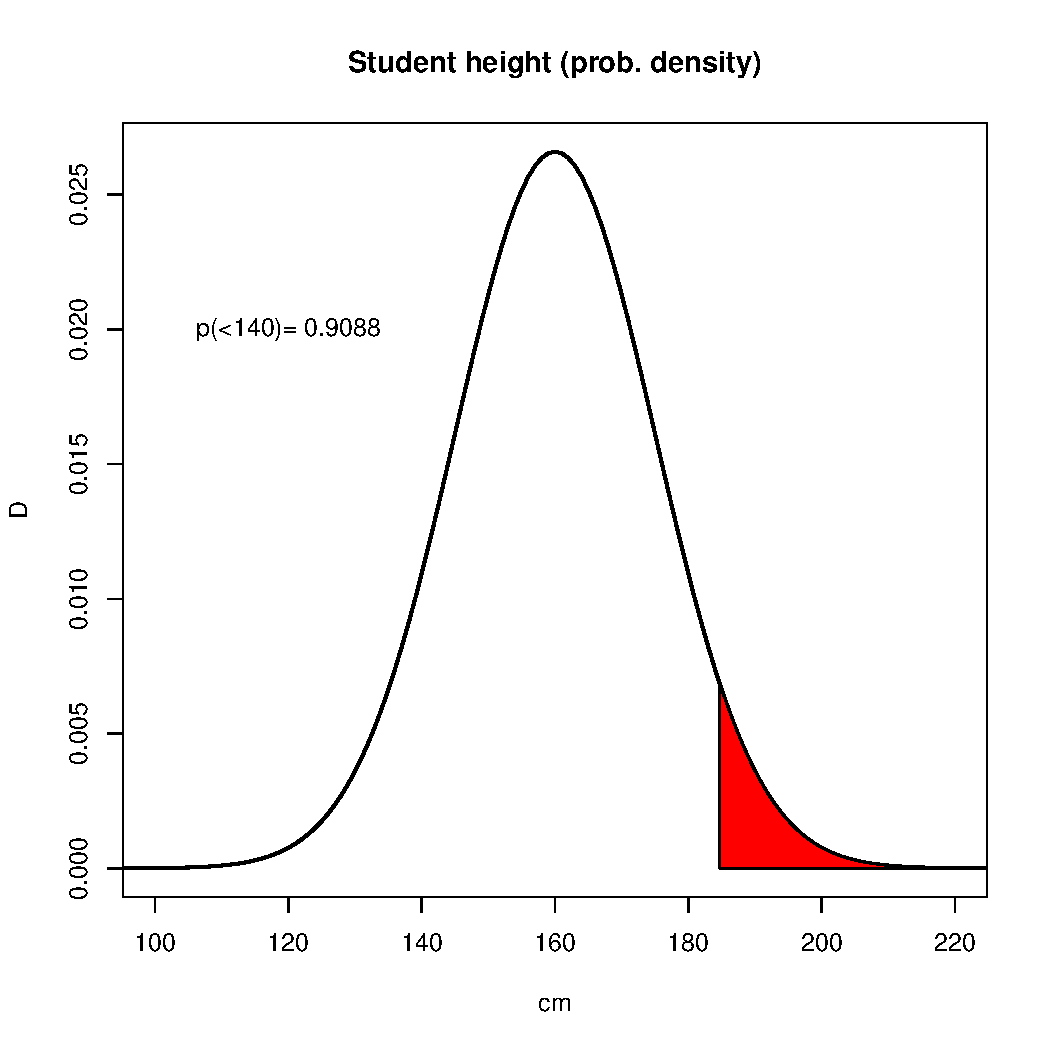
\includegraphics[width=\maxwidth]{figure/unnamed-chunk-16-1} 

\end{knitrout}
  \end{column}
\end{columns}
\end{frame}

%-----frame-----%
\begin{frame}[fragile]{Normal distribution}
\begin{columns}
  \begin{column}{0.5\textwidth}
  \begin{itemize}
    \item Continuous data ($\mu$ = mean, $\sigma$ = std.dev.)
    \item \texttt{r*}: random function, generates samples from the distribution
    \item E.g heights of 3 random students?
  \end{itemize}
\begin{knitrout}\scriptsize
\definecolor{shadecolor}{rgb}{0.969, 0.969, 0.969}\color{fgcolor}\begin{kframe}
\begin{alltt}
\hlkwd{rnorm}\hlstd{(}\hlnum{3}\hlstd{,} \hlnum{160}\hlstd{,} \hlnum{15}\hlstd{)}
\end{alltt}
\begin{verbatim}
## [1] 145.6133 168.2708 153.2355
\end{verbatim}
\begin{alltt}
\hlkwd{rnorm}\hlstd{(}\hlnum{3}\hlstd{,} \hlnum{160}\hlstd{,} \hlnum{15}\hlstd{)}
\end{alltt}
\begin{verbatim}
## [1] 143.2768 159.0669 166.8958
\end{verbatim}
\end{kframe}
\end{knitrout}
  \end{column}
  \begin{column}{0.5\textwidth}
\begin{knitrout}\scriptsize
\definecolor{shadecolor}{rgb}{0.969, 0.969, 0.969}\color{fgcolor}
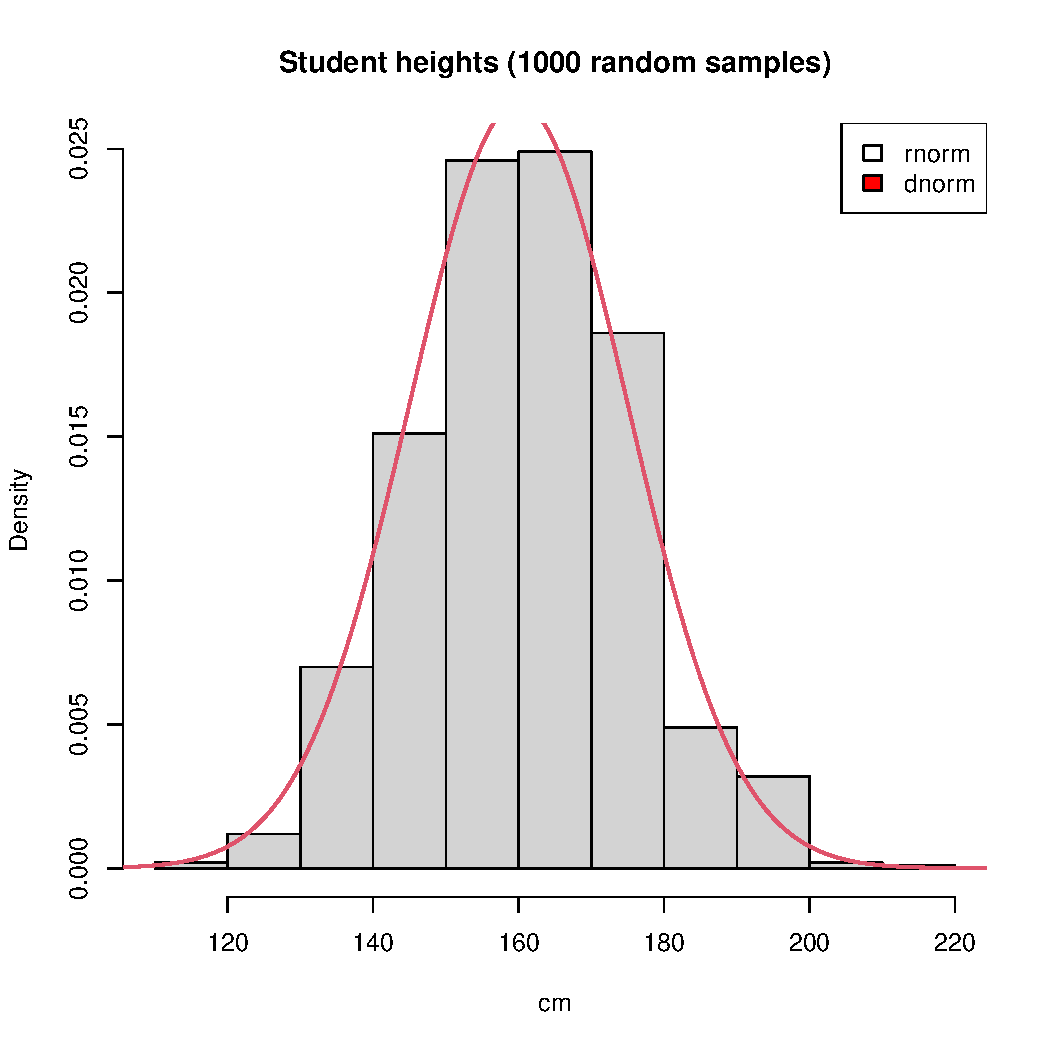
\includegraphics[width=\maxwidth]{figure/unnamed-chunk-18-1} 

\end{knitrout}
  \end{column}
\end{columns}
\end{frame}

\section{Statistical Inference}
%-----frame-----%
\begin{frame}{Statistical Inference}
Statistical Inference and hypothesis testing
\begin{itemize}
  \item Test some assumptions about a population of interest, using data drawn or sampled from that population
  \item Compared to descriptive statistics, inference gives significance of a statistical observation
  \item Examples
  \begin{itemize}
    \item Do two sets of observations have the same characteristics (mean, variance)?
    \item Are two variables correlated among a set of observations?
    \item Are observations distributed equally or not?
  \end{itemize}
\end{itemize}
\end{frame}

% %-----frame-----%
% \begin{frame}{Statistical Inference}
% \begin{itemize}
%   \item In general we wish to compare a statistic (e.g. mean) of a sample to a theoretical value or to another sample to look for differences
%   \item We use a \textit{test}-statistic to measure the difference, then compare this to a reference distribution of these statistics
%   \item The reference distribution tells us how much difference might be expected due to sample variation
%   \item If the observed statistic is much different from the expected range of values of the distribution, (i.e. does it fall in the tail-ends of the distribution) we might infer that the differences have not arisen by chance.
% \end{itemize}
% \end{frame}
% 
% %-----frame-----%
% \begin{frame}{Statistical Inference}
% \begin{itemize}
%   \item Choices to be made
%   \begin{itemize}
%     \item Which statistic (from descriptive statistic)?
%     \item Which reference distribution (of all possible values)?
%     \begin{itemize}
%       \item Theoretical
%       \item Empirical
%     \end{itemize}
%     \item What degree of certainty?
%     \begin{itemize}
%       \item Usually $<5\%$ of distribution?
%     \end{itemize}
%   \end{itemize}
% \end{itemize}
% \end{frame}
% 
\subsection{Student's $t$-test}
%-----frame-----%
\begin{frame}{Student's $t$-test}
\begin{columns}
  \begin{column}{0.75\textwidth}
  \begin{itemize}
    \item A $t$-test is used to compare an observed sample mean ($\mu_1$) to a hypothesized value ($\mu_{0}$) (one sample $t$-test)
    \item Or to compare two sample means (two sample $t$-test)
    %\item Answers the question: Is the difference in values ($\mu_1 - \mu_2$) large or small?
  \end{itemize}
  \begin{equation}
  t = \frac{\mu_1 - \mu_2}{s_{\mu_1-\mu2}}
  \end{equation}
  \begin{itemize}
    \item One-tailed ($\mu_1 < \mu_2$ or $\mu_1 > \mu_2$)
    \item Two-tailed ($\mu_1 \ne \mu_2$)
  \end{itemize}
  \end{column}
  \begin{column}{0.25\textwidth}
  \begin{center}
    	
\includegraphics[width=0.95\textwidth]{./images/guinnessbeer.png}
  \end{center}
  \end{column}
\end{columns}
\end{frame}

%-----frame-----%
\begin{frame}[fragile]{Student's $t$-test}

\begin{columns}
  \begin{column}{0.5\textwidth}
  \begin{center}
    	
\includegraphics[width=0.55\textwidth]{./images/Aragorn.png}
  \end{center}
  \begin{itemize}
    \item Two samples ($n=50$) of actors who auditioned for the role of Aragorn in Lord of the Rings in two different locations
    \item Is there a difference in heights?
  \end{itemize}
  \end{column}
  \begin{column}{0.5\textwidth}
\begin{knitrout}\scriptsize
\definecolor{shadecolor}{rgb}{0.969, 0.969, 0.969}\color{fgcolor}
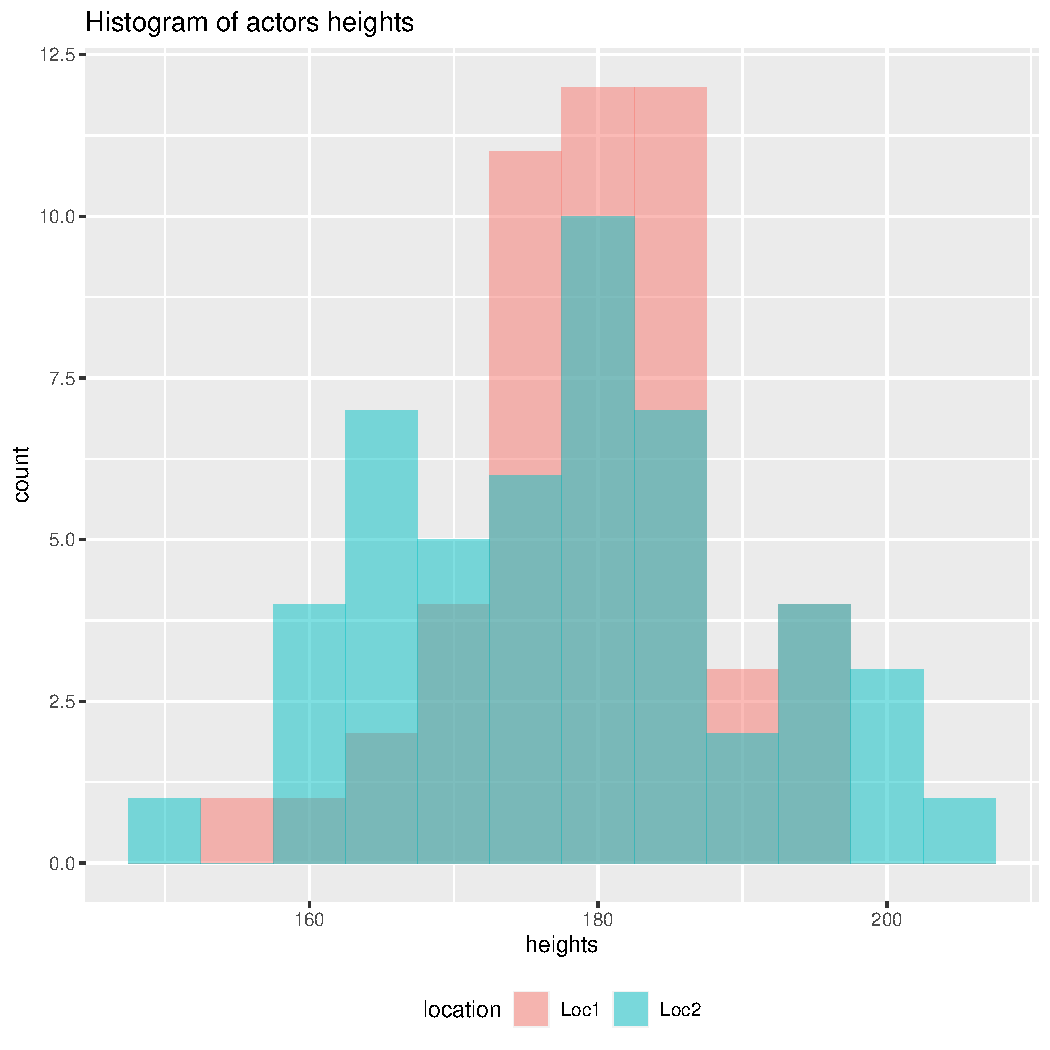
\includegraphics[width=\maxwidth]{figure/unnamed-chunk-20-1} 

\end{knitrout}
  \end{column}
\end{columns}
\end{frame}

%-----frame-----%
\begin{frame}[fragile]{Student's $t$-test}
\begin{columns}
  \begin{column}{0.5\textwidth}
  \begin{itemize}
    \item Is there a difference in mean height?
    \item Loc. 1 mean = 179.54
    \item Loc. 2 mean = 178.07
    \item Difference = 1.46
    \item $t$-statistic = 0.6886
  \end{itemize}
  \end{column}
  \begin{column}{0.5\textwidth}
\begin{knitrout}\scriptsize
\definecolor{shadecolor}{rgb}{0.969, 0.969, 0.969}\color{fgcolor}
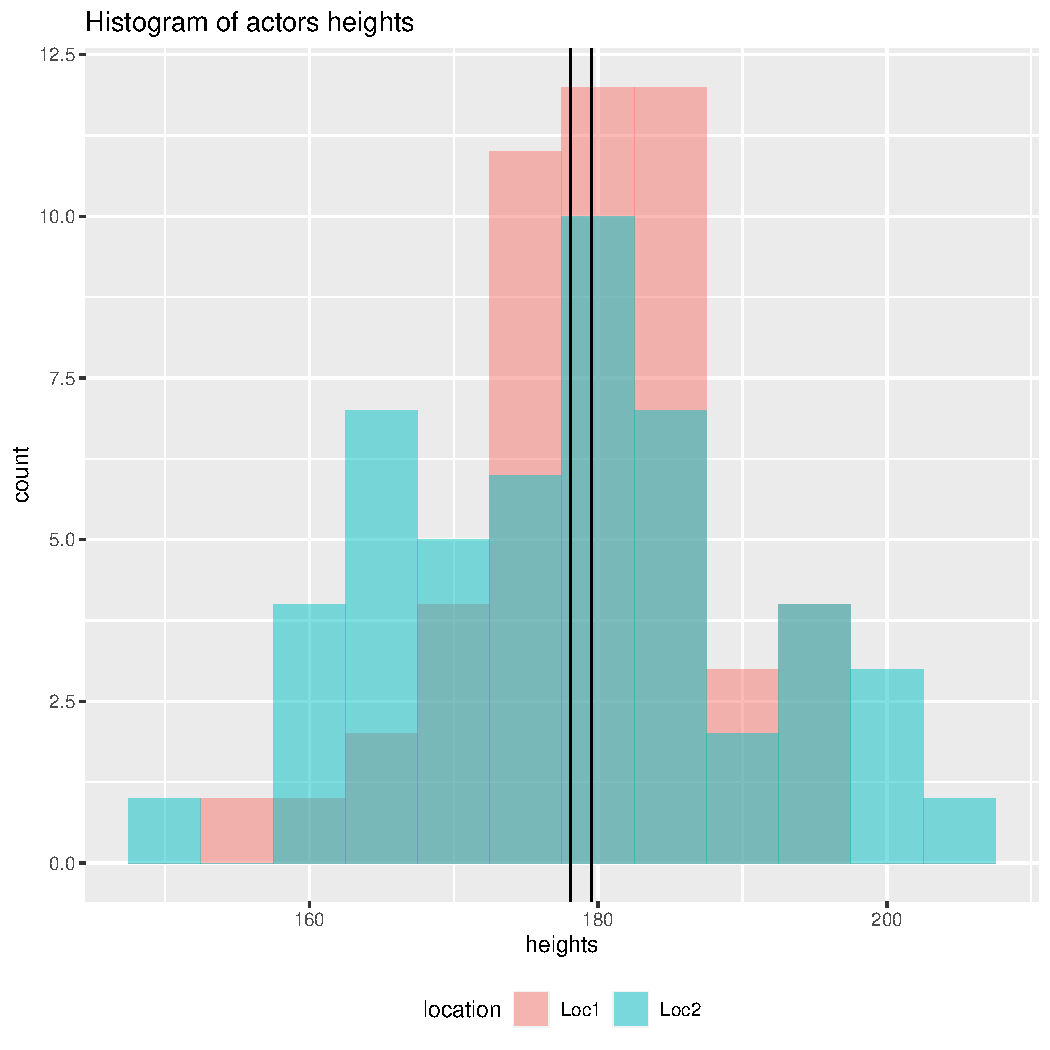
\includegraphics[width=\maxwidth]{figure/unnamed-chunk-21-1} 

\end{knitrout}
  \end{column}
\end{columns}
\end{frame}

%-----frame-----%
\begin{frame}[fragile]{Student's $t$-test}
\begin{columns}
  \begin{column}{0.5\textwidth}
  \begin{itemize}
    \item Compare $t$-statistic to $t$-distribution
    \item Represents the range of $t$-statistics expected through normal random variation
    \item If observed $t$ has a low probability (i.e. in one of the tails), it is less likely to have occured by chance ($p$-value)
    %\item The $p$-value represents the probability that this value (or larger) could have occurred by chance
    %\item Calculate as integral of distribution $<$ or $>$ this value
  \end{itemize}
  \end{column}
  \begin{column}{0.5\textwidth}
\begin{knitrout}\scriptsize
\definecolor{shadecolor}{rgb}{0.969, 0.969, 0.969}\color{fgcolor}
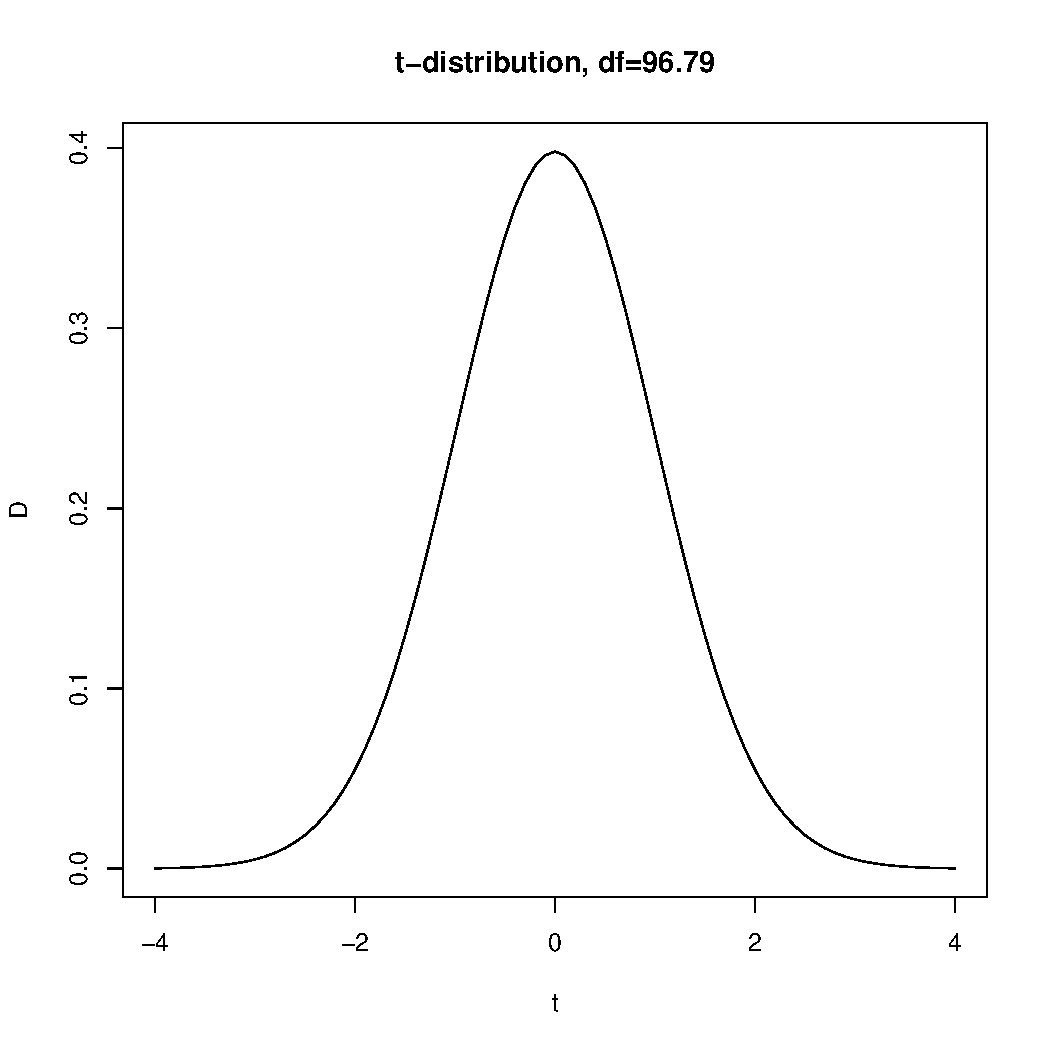
\includegraphics[width=\maxwidth]{figure/unnamed-chunk-22-1} 

\end{knitrout}
  \end{column}
\end{columns}
\end{frame}

% %-----frame-----%
% \begin{frame}[fragile]{Student's $t$-test}
% \begin{columns}
%   \begin{column}{0.5\textwidth}
%   \begin{itemize}
%     \item One-tail (greater than) test:
%     \item The $p$-value represents the probability that this value (or more) could have occurred by chance
%     \begin{itemize}
%       \item $p$-value is integral of curve $>$ $t$-statistic
%       \item $p$-value = round(t.test(apop1,apop2, alternative="greater")$p.value,4)
%     \end{itemize}
%   \end{itemize}
%   \end{column}
%   \begin{column}{0.5\textwidth}
% <<echo=FALSE>>=
% xt <- t.test(apop1,apop2)$statistic
% plot(qq,dt(qq,96.79), type='l', xlab="t", ylab="D", main="t-distribution, df=96.79")
% xvals <- seq(xt,4,length=100)
% dvals <- dt(xvals,96.79)
% polygon(c(xvals,rev(xvals)),c(rep(0,100),rev(dvals)),col="lightgray")
% @
%   \end{column}
% \end{columns}
% \end{frame}
% 
% %-----frame-----%
% \begin{frame}[fragile]{Student's $t$-test}
% $t$-test in R using the \texttt{t.test()} function:
% <<echo=TRUE>>=
% t.test(apop1, apop2, alternative = "greater")
% @
% \end{frame}
% 
% %-----frame-----%
% \begin{frame}[fragile]{Student's $t$-test}
% \begin{columns}
%   \begin{column}{0.5\textwidth}
%   \begin{itemize}
%     \item One-tail (lesser than) test:
%     \item The $p$-value represents the probability that this value (or less) could have occurred by chance
%     \item One-tail test:
%     \begin{itemize}
%       \item $p$-value is integral of curve $<$ $t$-statistic
%       \item $p$-value = round(t.test(apop1,apop2, alternative="less")$p.value,4)
%     \end{itemize}
%   \end{itemize}
%   \end{column}
%   \begin{column}{0.5\textwidth}
% <<echo=FALSE>>=
% xt <- t.test(apop1,apop2)$statistic
% plot(qq,dt(qq,96.79), type='l', xlab="t", ylab="D", main="t-distribution, df=96.79")
% xvals <- seq(-4,xt,length=100)
% dvals <- dt(xvals,96.79)
% polygon(c(xvals,rev(xvals)),c(rep(0,100),rev(dvals)),col="lightgray")
% @
%   \end{column}
% \end{columns}
% \end{frame}
% 
% %-----frame-----%
% \begin{frame}[fragile]{Student's $t$-test}
% $t$-test in R using the \texttt{t.test()} function:
% <<echo=TRUE>>=
% t.test(apop1, apop2, alternative = "less")
% @
% \end{frame}
% 
%-----frame-----%
\begin{frame}[fragile]{Student's $t$-test}
\begin{columns}
  \begin{column}{0.5\textwidth}
  \begin{itemize}
    \item Two-tail test:
    \item The $p$-value represents the probability that this \emph{difference} (positive or negative) could have occurred by chance
    \begin{itemize}
      \item $p$-value is integral of curve $< -|t|$ plus integral of curve $> |t|$
      \item $p$-value = 0.4929
    \end{itemize}
  \end{itemize}
  \end{column}
  \begin{column}{0.5\textwidth}
\begin{knitrout}\scriptsize
\definecolor{shadecolor}{rgb}{0.969, 0.969, 0.969}\color{fgcolor}
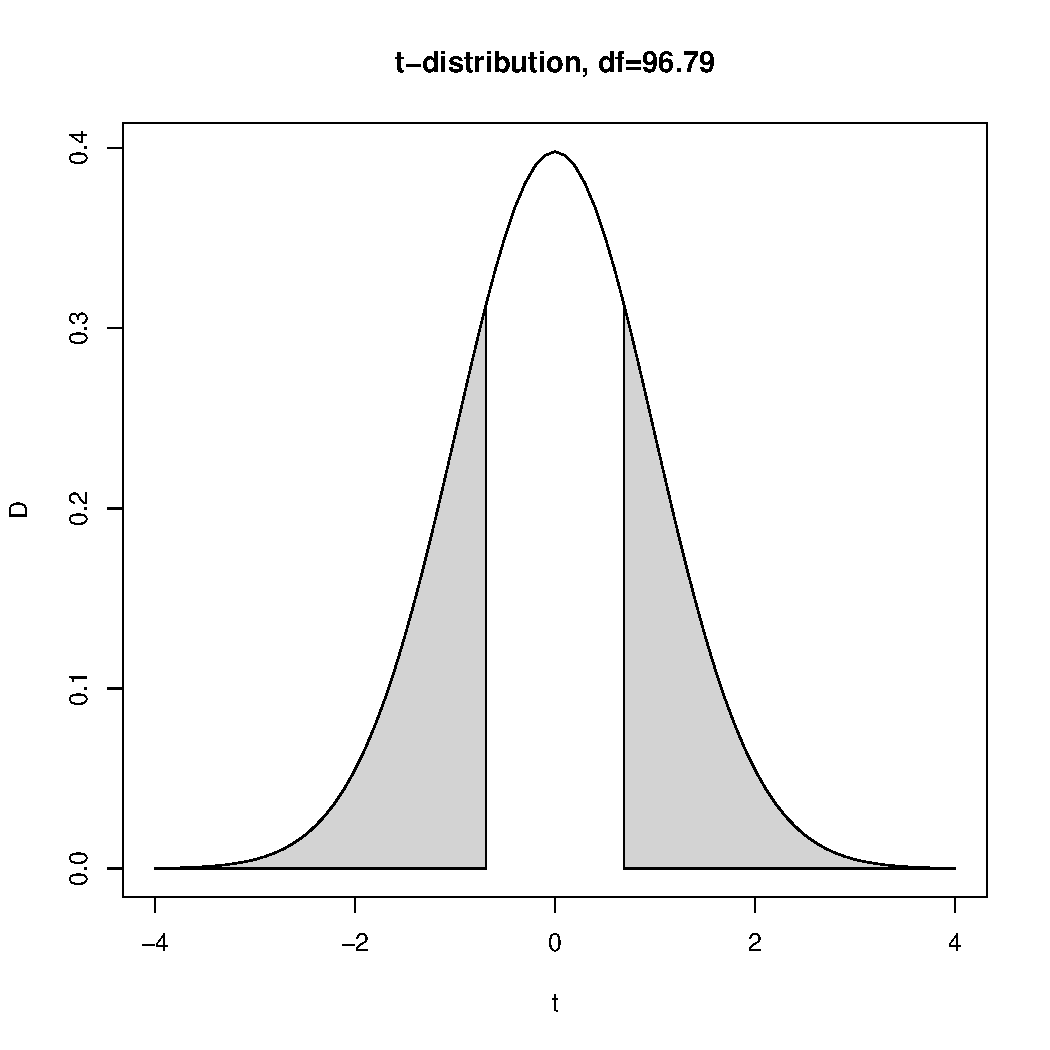
\includegraphics[width=\maxwidth]{figure/unnamed-chunk-23-1} 

\end{knitrout}
  \end{column}
\end{columns}
\end{frame}

%-----frame-----%
\begin{frame}[fragile]{Student's $t$-test}
$t$-test in R using the \texttt{t.test()} function:
\begin{knitrout}\scriptsize
\definecolor{shadecolor}{rgb}{0.969, 0.969, 0.969}\color{fgcolor}\begin{kframe}
\begin{alltt}
\hlkwd{t.test}\hlstd{(apop1, apop2,} \hlkwc{alternative} \hlstd{=} \hlstr{"two.sided"}\hlstd{)}
\end{alltt}
\begin{verbatim}
## 
## 	Welch Two Sample t-test
## 
## data:  apop1 and apop2
## t = 0.68864, df = 87.394, p-value = 0.4929
## alternative hypothesis: true difference in means is not equal to 0
## 95 percent confidence interval:
##  -2.761618  5.690039
## sample estimates:
## mean of x mean of y 
##  179.5392  178.0750
\end{verbatim}
\end{kframe}
\end{knitrout}
\end{frame}

%-----frame-----%
\begin{frame}[fragile]{Student's $t$-test}

\begin{columns}
  \begin{column}{0.5\textwidth}
  \begin{itemize}
    \item If we also had 50 actors who auditioned for Gimli + 50 who auditioned for Aragorn
    \item Difference = 22.48
    \item $t$-statistic = 9.2512
  \end{itemize}
  \begin{center}
      
\includegraphics[width=0.55\textwidth]{./images/Gimli.jpg}
  \end{center}
  \end{column}
  \begin{column}{0.5\textwidth}
\begin{knitrout}\scriptsize
\definecolor{shadecolor}{rgb}{0.969, 0.969, 0.969}\color{fgcolor}
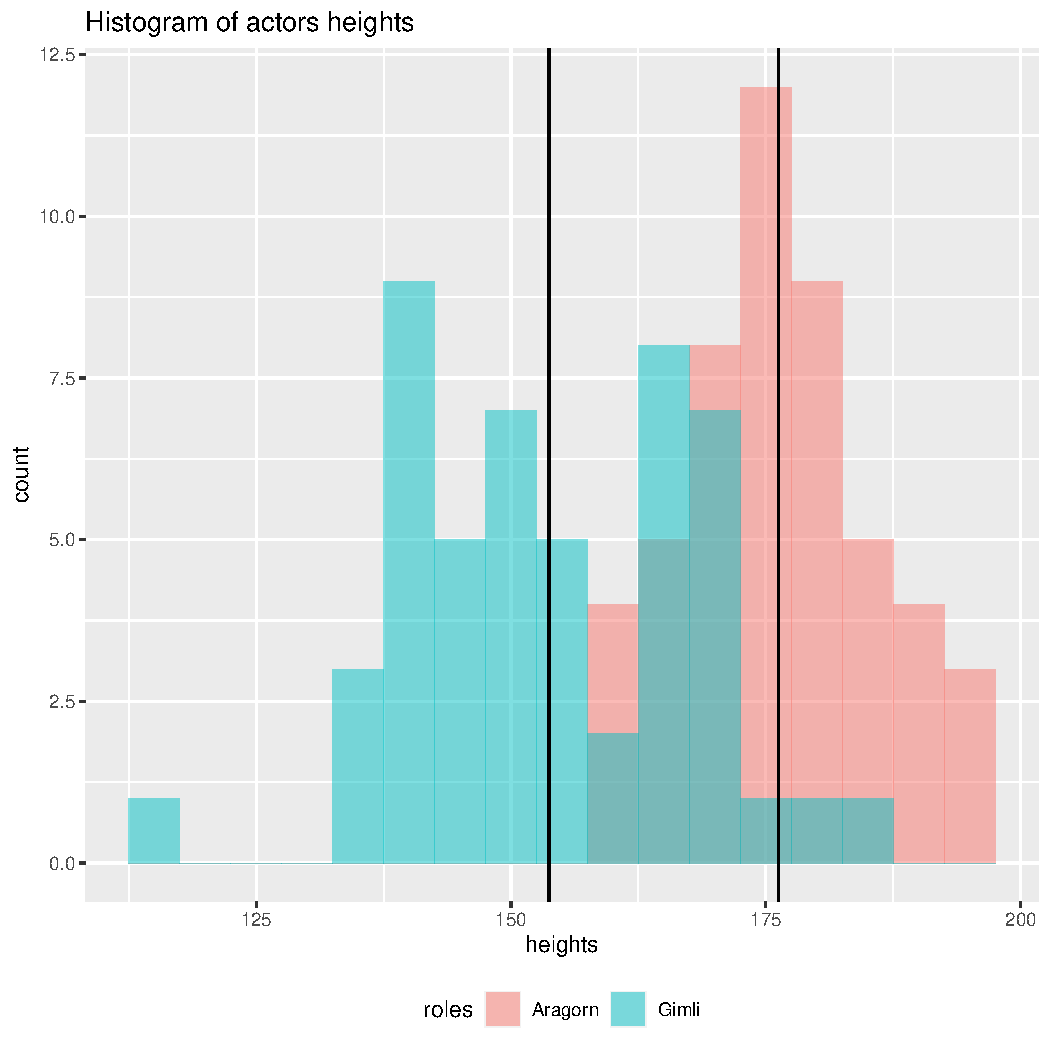
\includegraphics[width=\maxwidth]{figure/unnamed-chunk-26-1} 

\end{knitrout}
  \end{column}
\end{columns}
\end{frame}

%-----frame-----%
\begin{frame}[fragile]{Student's $t$-test}
\begin{columns}
  \begin{column}{0.5\textwidth}
  \begin{itemize}
    \item The $p$-value represents the probability that this value (or larger) could have occurred by chance
    \item Two-tail test:
    \begin{itemize}
      \item $p$-value is integral of curve $< -|t|$ plus integral of curve $> |t|$
      \item $p$-value = \ensuremath{1.4492108\times 10^{-14}}
    \end{itemize}
  \end{itemize}
  \end{column}
  \begin{column}{0.5\textwidth}
\begin{knitrout}\scriptsize
\definecolor{shadecolor}{rgb}{0.969, 0.969, 0.969}\color{fgcolor}
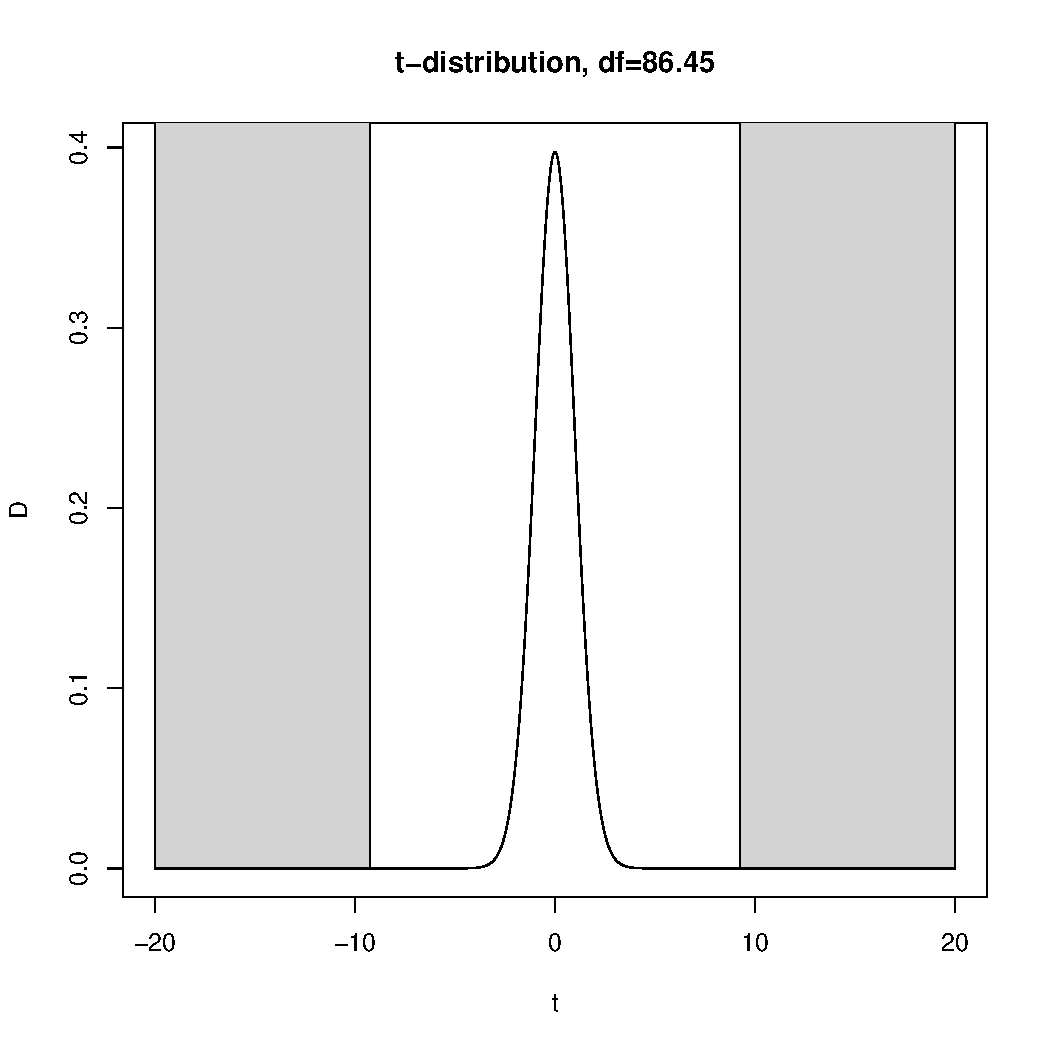
\includegraphics[width=\maxwidth]{figure/unnamed-chunk-27-1} 

\end{knitrout}
  \end{column}
\end{columns}
\end{frame}

%-----frame-----%
\begin{frame}[fragile]{Student's $t$-test}
$t$-test in R using the \texttt{t.test()} function:
\begin{knitrout}\scriptsize
\definecolor{shadecolor}{rgb}{0.969, 0.969, 0.969}\color{fgcolor}\begin{kframe}
\begin{alltt}
\hlkwd{t.test}\hlstd{(aragorn, gimli,} \hlkwc{alternative} \hlstd{=} \hlstr{"two.sided"}\hlstd{)}
\end{alltt}
\begin{verbatim}
## 
## 	Welch Two Sample t-test
## 
## data:  aragorn and gimli
## t = 9.2512, df = 86.451, p-value = 1.449e-14
## alternative hypothesis: true difference in means is not equal to 0
## 95 percent confidence interval:
##  17.64770 27.30697
## sample estimates:
## mean of x mean of y 
##  176.2119  153.7345
\end{verbatim}
\end{kframe}
\end{knitrout}
\end{frame}

%-----frame-----%
\begin{frame}[fragile]{Student's $t$-test}
$t$-test in R using the \texttt{t.test()} function (one-sided):
\begin{knitrout}\scriptsize
\definecolor{shadecolor}{rgb}{0.969, 0.969, 0.969}\color{fgcolor}\begin{kframe}
\begin{alltt}
\hlkwd{t.test}\hlstd{(aragorn, gimli,} \hlkwc{alternative} \hlstd{=} \hlstr{"greater"}\hlstd{)}
\end{alltt}
\begin{verbatim}
## 
## 	Welch Two Sample t-test
## 
## data:  aragorn and gimli
## t = 9.2512, df = 86.451, p-value = 7.246e-15
## alternative hypothesis: true difference in means is greater than 0
## 95 percent confidence interval:
##  18.43762      Inf
## sample estimates:
## mean of x mean of y 
##  176.2119  153.7345
\end{verbatim}
\end{kframe}
\end{knitrout}
\end{frame}

\subsection{ANOVA}
%-----frame-----%
\begin{frame}[fragile]{ANOVA}

\begin{columns}
  \begin{column}{0.5\textwidth}
  \begin{itemize}
    \item What if we have more than two groups?
    \item If we also have 50 actors who auditioned for Legolas
  \end{itemize}
  \begin{center}
      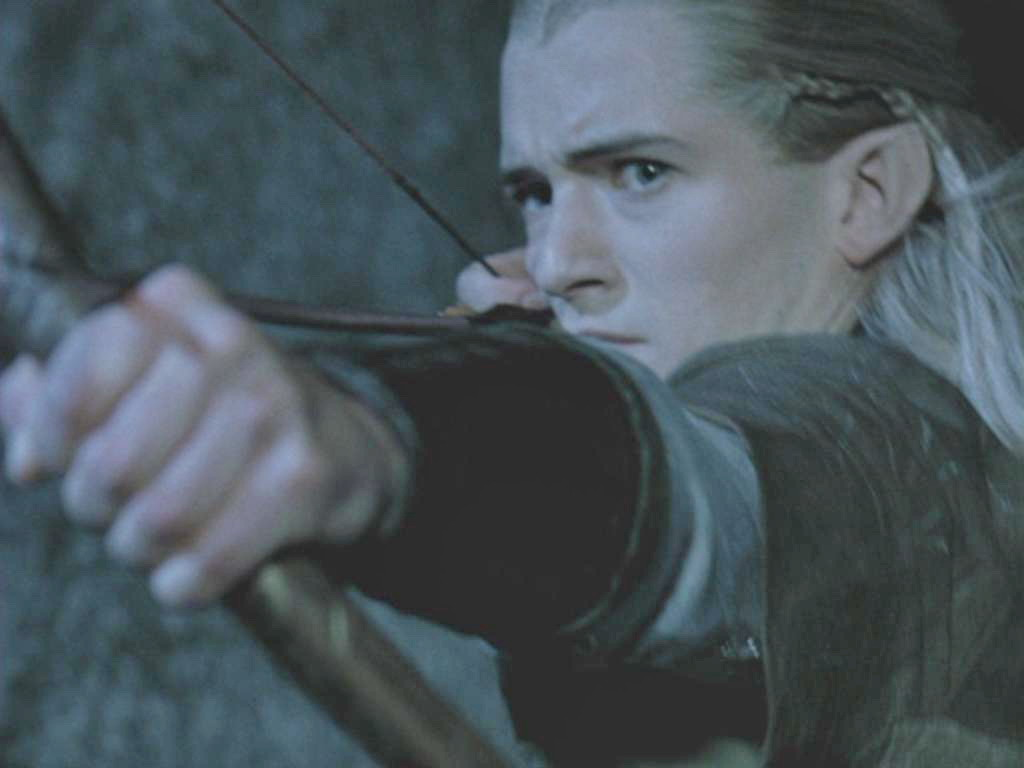
\includegraphics[width=0.55\textwidth]{./images/Legolas.jpg}
  \end{center}
  \end{column}
  \begin{column}{0.5\textwidth}
\begin{knitrout}\scriptsize
\definecolor{shadecolor}{rgb}{0.969, 0.969, 0.969}\color{fgcolor}
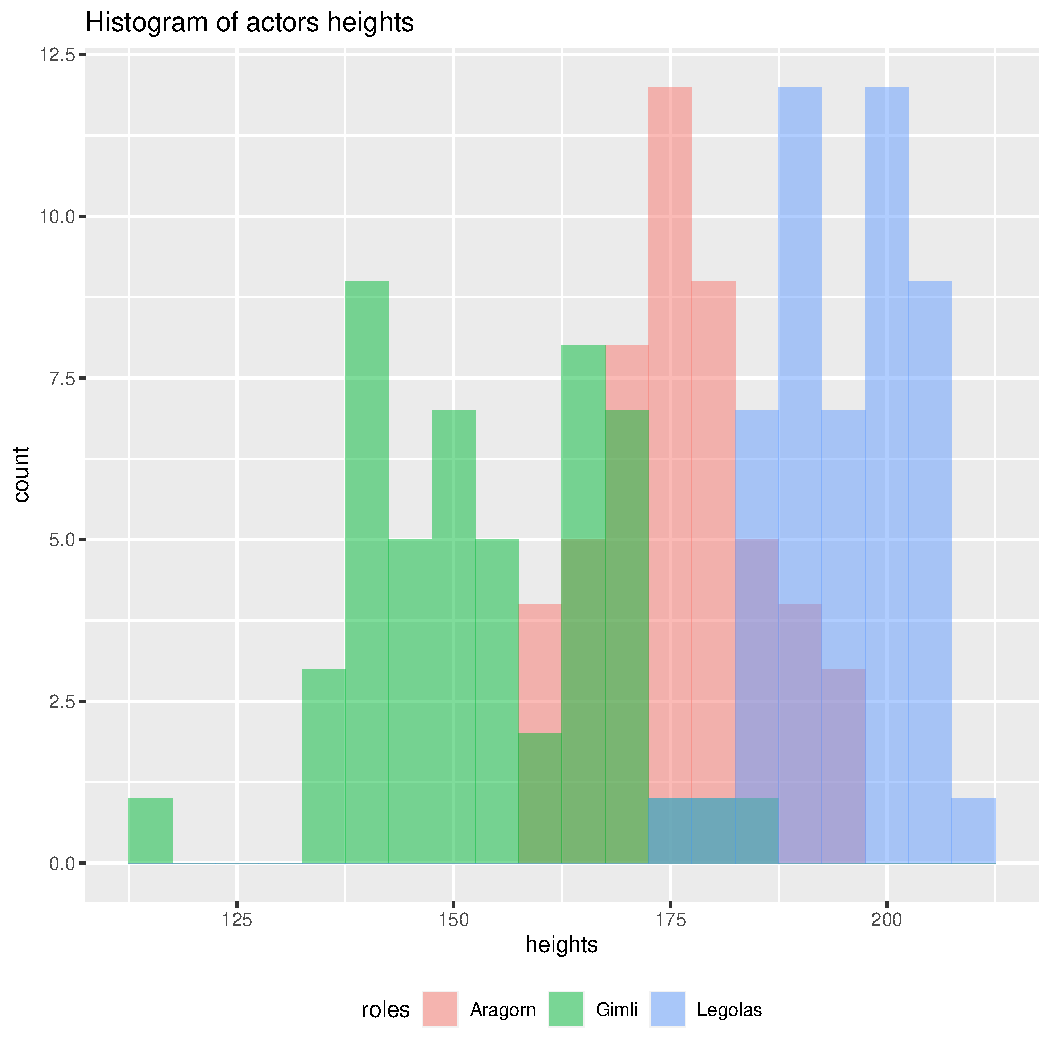
\includegraphics[width=\maxwidth]{figure/unnamed-chunk-31-1} 

\end{knitrout}
  \end{column}
\end{columns}
\end{frame}

% %--- Slide ----------------%
% \begin{frame}{ANOVA}
% Analysis of variance --- ANOVA
% \begin{itemize}
%   \item ANOVA can be used to compare the means of two or more groups 
% 	\item Extension of the $t$-test for differences of the means of two groups, but different approach
% 	\item Uses the variances of the observations to compare means
% 	\item Has additional uses in regression analysis
% 	\item $H_0$ --- there is no difference between the $n$ groups
% 	\item $H_a$ --- at least one of the $n$ groups has a different mean
% \end{itemize}
% \end{frame}
% 
% %--- Slide ----------------%
% % \begin{frame}{ANOVA}
% % 	\begin{center}
% % 		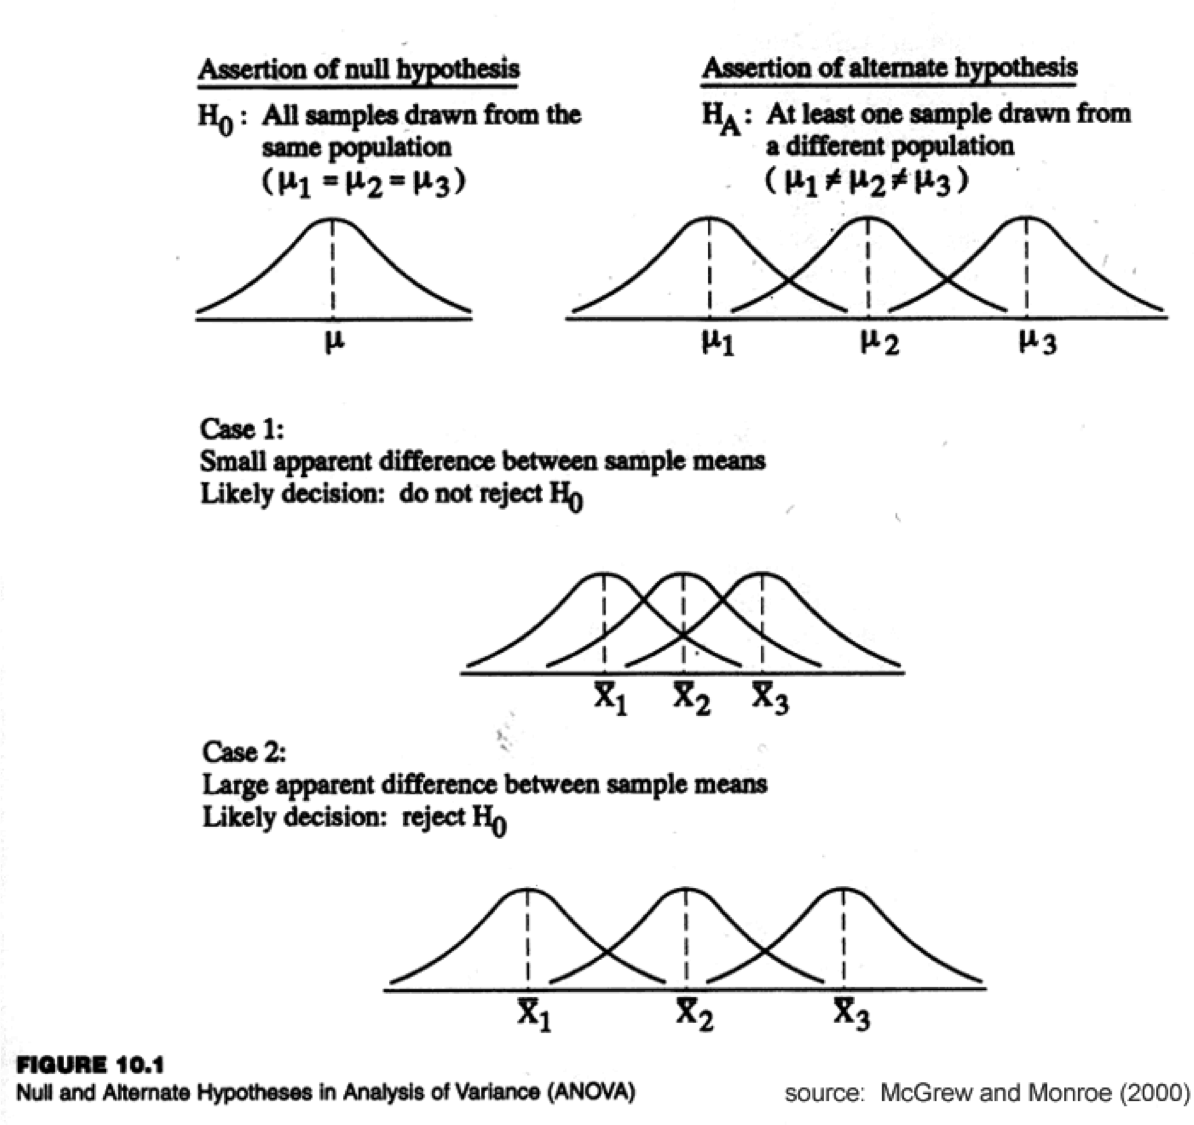
\includegraphics[width=0.7\textwidth]{./images/aov.png}
% % 	\end{center}
% % \end{frame}
% 
% %--- Slide ----------------%
% \begin{frame}{ANOVA}
% Calculation of ANOVA by variance decomposition
% \begin{itemize}
% 	\item Samples have a total variance $\sigma^2$
% 	\item Knowing group membership, the contribution of any observation $x_{ij}$ to this variance can be split into two parts
% \end{itemize}
% \begin{equation}
% 	(x_{ij} - \bar{x}) = (\bar{x_i} - \bar{x}) + (x_{ij} - \bar{x_i})
% \end{equation}
% \begin{itemize}
% 	\item Where $x_{ij}$ is the value for observation $j$; $\bar{x_i}$ is the mean of a given group $i$; $\bar{x}$ is the overall mean
% \end{itemize}
% \end{frame}
% 
% %--- Slide ----------------%
% \begin{frame}{ANOVA}
% Decomposition of variance for a dataset with three groups
% 	\begin{center}
% 		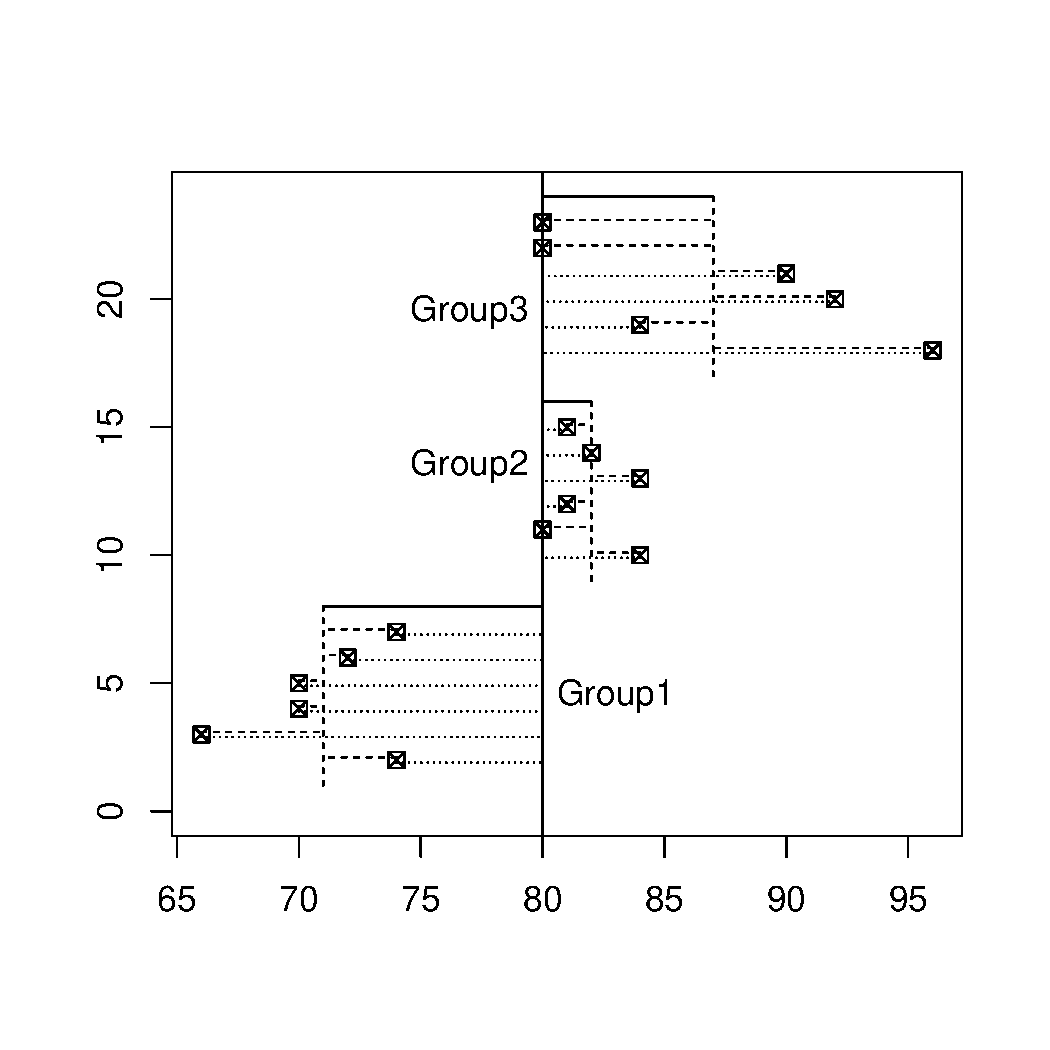
\includegraphics[width=0.6\textwidth]{./images/sourcesofvariance}
% 	\end{center}
% \end{frame}
% 
% %--- Slide ----------------%
% \begin{frame}{ANOVA}
% We now square and sum the differences for each observations as follow
% \begin{equation}
% 	\sum_{i=1}^{t} \sum_{j=1}^{n} (x_{ij} - \bar{x})^2 = 
% 	n \sum_{i=1}^{t} (\bar{x_i} - \bar{x})^2 + 
% 	\sum_{i=1}^{t} \sum_{j=1}^{n} (x_{ij} - \bar{x_i})^2
% \end{equation}
% \emph{Total} variation or \emph{sum of squares} may be split into \emph{between} and
% \emph{error} components. 
% Frequently written as:
% \begin{equation}
% 	TSS = BSS + ESS
% \end{equation}
% \end{frame}

%--- Slide ----------------%
\begin{frame}{ANOVA}
The $F$-statistic is used to test for significance in the split of variance:
\begin{equation}
		F = \frac{BSS/(t-1)}{ESS/(n-t-1)} 
\end{equation}
\begin{itemize}
	\item Ratio of how much of the variance is between the groups to how much is within the groups
	\item Compare to an $F$-distribution, using degrees of freedom based on the number of groups ($t$) and the number of observations ($n$)
\end{itemize}
\end{frame}

%-----frame-----%
\begin{frame}[fragile]{ANOVA}
  \begin{itemize}
    \item We can use the R function \texttt{aov()} to calculate ANOVA for the three groups. Note this uses the model syntax ($\sim$)
  \end{itemize}
\begin{knitrout}\scriptsize
\definecolor{shadecolor}{rgb}{0.969, 0.969, 0.969}\color{fgcolor}\begin{kframe}
\begin{alltt}
\hlstd{roles} \hlkwb{=} \hlkwd{c}\hlstd{(}\hlkwd{rep}\hlstd{(}\hlstr{"Aragorn"}\hlstd{,}\hlnum{50}\hlstd{),} \hlkwd{rep}\hlstd{(}\hlstr{"Gimli"}\hlstd{,}\hlnum{50}\hlstd{),} \hlkwd{rep}\hlstd{(}\hlstr{"Legolas"}\hlstd{,}\hlnum{50}\hlstd{))}
\hlstd{heights} \hlkwb{=} \hlkwd{c}\hlstd{(aragorn, gimli, legolas)}
\hlkwd{summary}\hlstd{(}\hlkwd{aov}\hlstd{(heights} \hlopt{~} \hlstd{roles))}
\end{alltt}
\begin{verbatim}
##              Df Sum Sq Mean Sq F value Pr(>F)    
## roles         2  42767   21383   181.5 <2e-16 ***
## Residuals   147  17319     118                   
## ---
## Signif. codes:  0 '***' 0.001 '**' 0.01 '*' 0.05 '.' 0.1 ' ' 1
\end{verbatim}
\end{kframe}
\end{knitrout}
\end{frame}

\section{Other inference tests}
%-----frame-----%
\begin{frame}{Other inference tests}
\begin{itemize}
  \item $F$-test: test if difference in ratio of variance of two samples
  \begin{itemize}
    \item \texttt{var.test()}
  \end{itemize}
  \item Wilcoxon rank sum test: Non-parametric test for the equality of medians 
  \begin{itemize}
    \item \texttt{wilcox.test()}
  \end{itemize}
  \item Correlation tests: tests of \emph{covariation}
  \begin{itemize}
    \item \texttt{cor.test()}
    \item Pearson's vs. Spearman's
  \end{itemize}
  \item Chi-squared ($\chi^2$) tests: tests of \emph{distribution} and \emph{association}
  \begin{itemize}
    \item \texttt{chisq.test()}
  \end{itemize}
\end{itemize}
\end{frame}

% %--- Slide ----------------%
% \begin{frame}{Next Class}
% \begin{itemize}
%   \item 0302: Extending R with addon packages
%   \item Lab: Inference tests in R
% \end{itemize}
% \end{frame}
% 
\end{document}
